% Chinese translation assembled from source/blocks.json.

% See source/translation.py for the translation and source/build_tex.py for assembly.

% source-block: 271211a5-58b7-80b8-9a51-c4976dca1254 (header; source-index: 137)

\hypertarget{src-271211a5-58b7-80b8-9a51-c4976dca1254}{}
\section*{4. 缓解训练与推理不匹配的尝试}
\phantomsection
\addcontentsline{toc}{section}{4. 缓解训练与推理不匹配的尝试}


% source-block: 271211a5-58b7-8025-aee7-c19ceda8ac80 (text; source-index: 138)

下面列出我们尝试过的缓解方法。其中有些有效，有些没有奏效。


% source-block: 271211a5-58b7-80f7-beba-e43453ed1380 (sub_header; source-index: 139)

\hypertarget{src-271211a5-58b7-80f7-beba-e43453ed1380}{}
\subsection*{4.1 未奏效的尝试}
\phantomsection
\addcontentsline{toc}{subsection}{4.1 未奏效的尝试}


% source-block: 271211a5-58b7-80c3-96aa-ed277ca67b21 (sub_sub_header; source-index: 140)

\hypertarget{src-271211a5-58b7-80c3-96aa-ed277ca67b21}{}
\subsubsection*{4.1.1 使用 FP32 语言模型输出头}


% source-block: 271211a5-58b7-802d-a418-e2b9da375651 (text; source-index: 141)

受 \href{https://arxiv.org/abs/2506.13585}{MiniMax-M1 技术报告}和博客\href{https://fengyao.notion.site/off-policy-rl}{《高效的强化学习框架暗中将训练变成了异策略强化学习》}启发，我们修改 vLLM，将 \code{lm_head} 转为 FP32 精度。然而，修改后不匹配仍然存在，模型崩溃依旧无法避免。图 11 对比了 L20 上使用 BF16 \code{lm_head} 的失败同策略实验，以及从该失败实验第 200 步恢复、改用 FP32 \code{lm_head} 的实验。两次实验最终都崩溃了，使用 FP32 \code{lm_head} 的实验仍出现了 \code{vllm-kl} 爆炸。


% source-block: 271211a5-58b7-80d3-98ac-fe024795f621 (image; source-index: 142)

\begin{figure}[H]
\centering
% source-block: 271211a5-58b7-80d3-98ac-fe024795f621 (image)
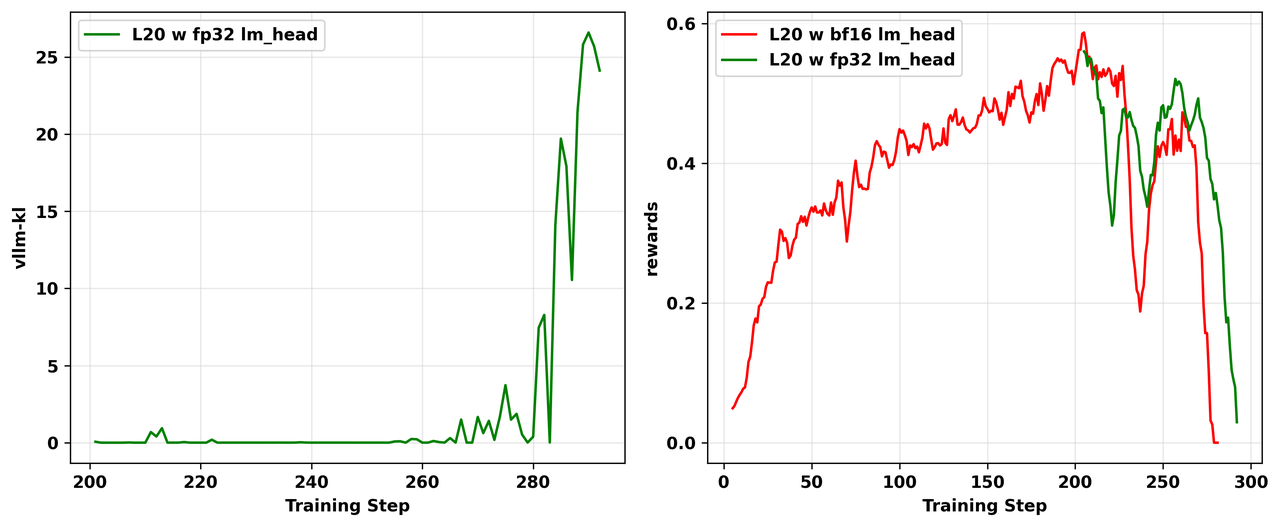
\includegraphics[width=\linewidth,height=0.64\textheight,keepaspectratio]{figures/image-17.png}
\caption*{\textbf{图 11。}vLLM 引擎中 \code{lm_head} 精度的消融实验。左：\code{vllm-kl}；右：训练奖励。使用 FP32 \code{lm_head} 的实验，从 BF16 \code{lm_head} 失败实验的第 200 步恢复。}
\end{figure}


% source-block: 277211a5-58b7-8065-8a78-def969cdd1ca (divider; source-index: 143)

% source-block: 271211a5-58b7-80ee-960c-f43a87c9177a (sub_sub_header; source-index: 144)

\hypertarget{src-271211a5-58b7-80ee-960c-f43a87c9177a}{}
\subsubsection*{4.1.2 关闭分块预填充}


% source-block: 271211a5-58b7-804e-b961-ec63fb9bf0a5 (text; source-index: 145)

我们还从第 4.1.1 节中使用 BF16 \code{lm_head} 的失败实验第 200 步恢复训练，尝试关闭\href{https://docs.vllm.ai/en/v0.4.2/models/performance.html}{分块预填充（chunked prefill）}，检验能否解决崩溃。图 12 表明，这一方法没有解决问题。


% source-block: 271211a5-58b7-8054-8c5b-d9ce67ee4d3d (image; source-index: 146)

\begin{figure}[H]
\centering
% source-block: 271211a5-58b7-8054-8c5b-d9ce67ee4d3d (image)
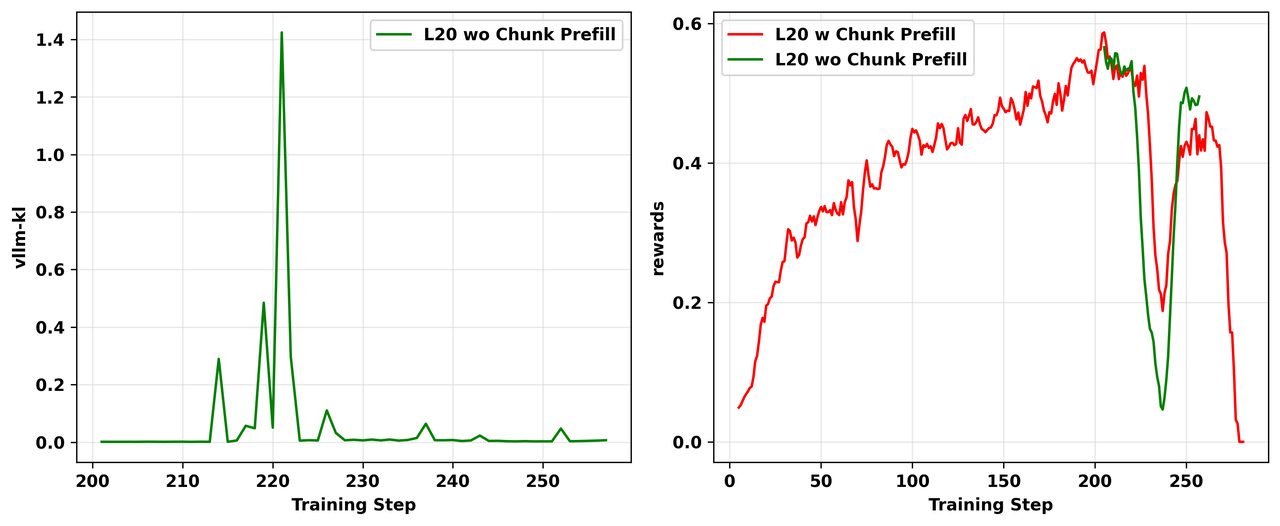
\includegraphics[width=\linewidth,height=0.64\textheight,keepaspectratio]{figures/image-18.png}
\caption*{\textbf{图 12。}分块预填充的消融实验。从此前启用分块预填充的失败实验第 200 步恢复训练，并关闭该功能。左：\code{vllm-kl}；右：训练奖励。}
\end{figure}


% source-block: 271211a5-58b7-8079-881a-cb3f4f1ef2c6 (sub_sub_header; source-index: 147)

\hypertarget{src-271211a5-58b7-8079-881a-cb3f4f1ef2c6}{}
\subsubsection*{4.1.3 启用 \texttt{enforce\_eager} 和 \texttt{free\_cache\_engine}}


% source-block: 271211a5-58b7-80f3-a489-f51061ca6f89 (text; source-index: 148)

\href{https://verl.readthedocs.io/en/latest/algo/dapo.html}{VeRL 的 DAPO 官方配方}提到，启用 CUDA Graph（\code{enforce_eager=False}，原文此处拼作 \code{enforce_eage}）可能导致模型性能下降。为研究它是否影响训练与推理不匹配，我们同时考虑另一个超参数 \code{free_cache_engine}，开展消融实验。

实验采用推理强化学习设置：在 H100 GPU 上，以 Qwen3-4B-Base 为基础模型运行同策略 GRPO，将 \code{enforce_eager} 与 \code{free_cache_engine} 分别设为 \code{True} 或 \code{False}，穷举四种组合，并在 AIME24 上评估。图 13 表明，调整这两个参数，对训练与推理不匹配以及测试性能均没有显著影响。


% source-block: 271211a5-58b7-8084-b459-d4cd5f78014f (image; source-index: 149)

\begin{figure}[H]
\centering
% source-block: 271211a5-58b7-8084-b459-d4cd5f78014f (image)
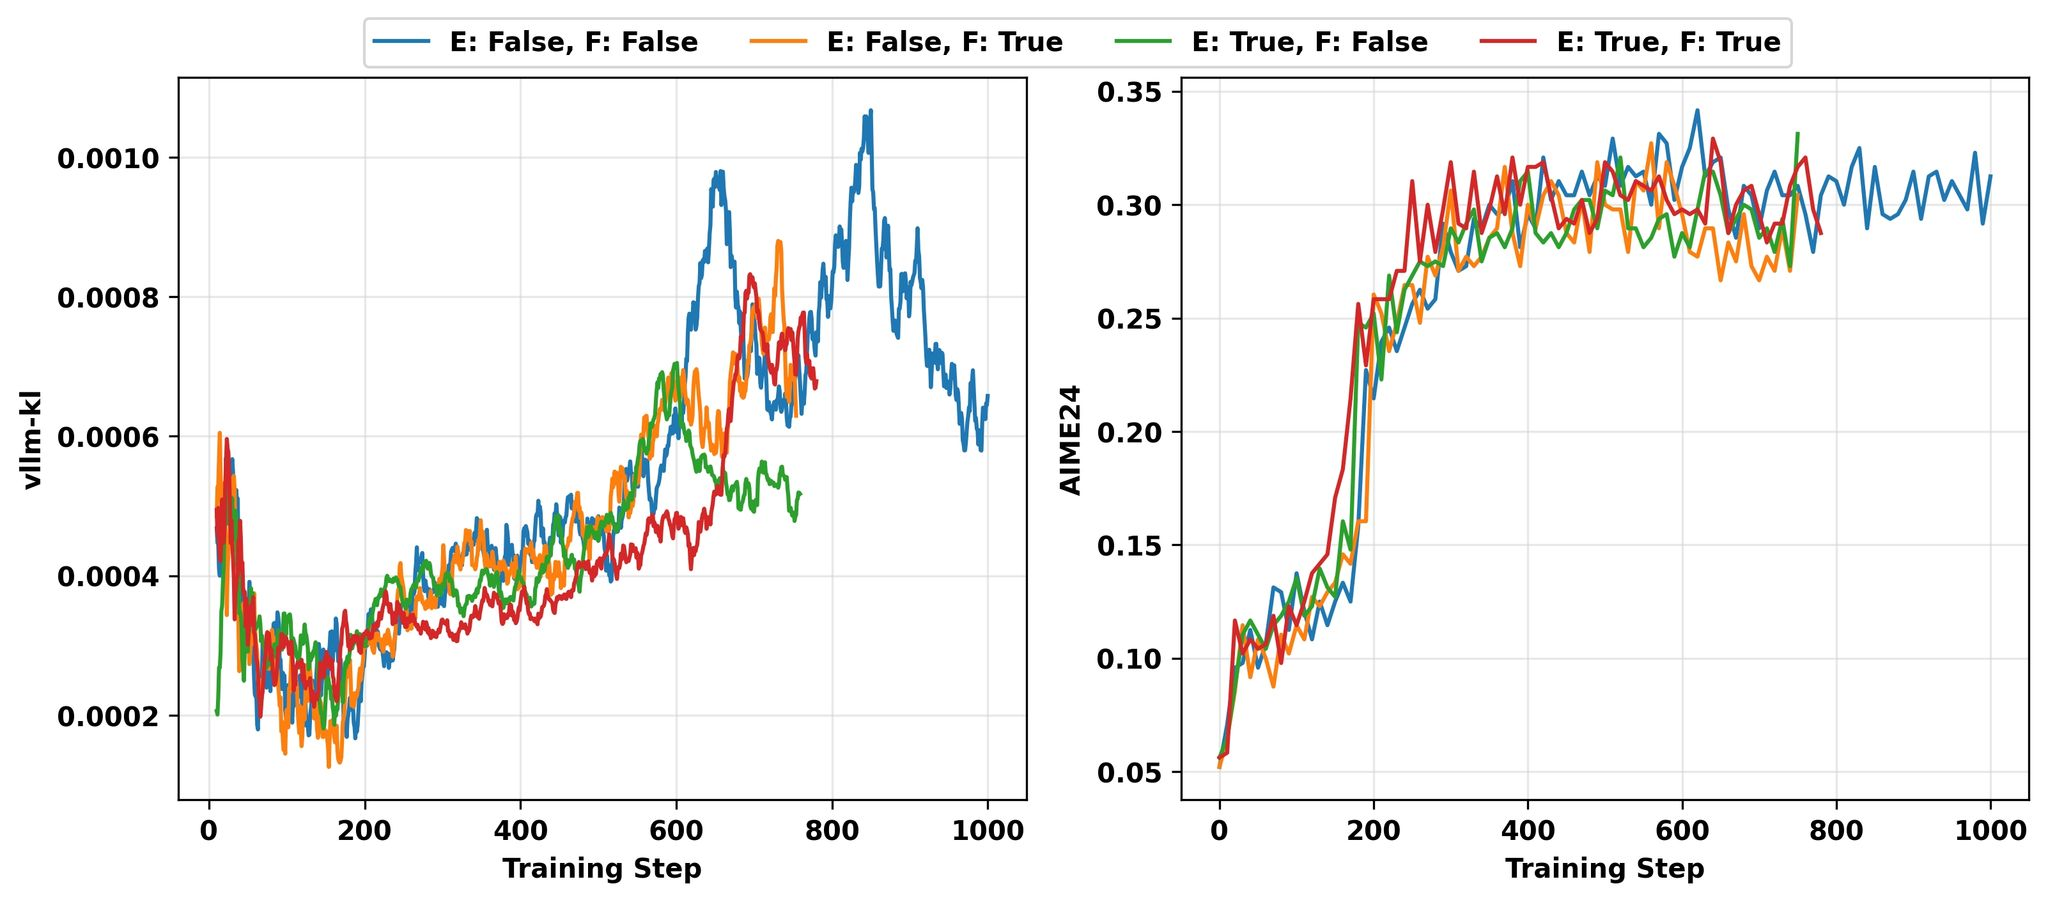
\includegraphics[width=\linewidth,height=0.64\textheight,keepaspectratio]{figures/image-19.jpg}
\caption*{\textbf{图 13。}推理强化学习中，vLLM 加速与缓存相关超参数的消融实验。在 H100 上运行同策略 GRPO，穷举 \code{enforce_eager}（E）与 \code{free_cache_engine}（F）的四种组合。左：\code{vllm-kl}；右：AIME24 准确率。}
\end{figure}


% source-block: 277211a5-58b7-8090-b5aa-dfaba7160a2c (divider; source-index: 150)

% source-block: 271211a5-58b7-801e-bd8e-d67fd96e9ee5 (sub_header; source-index: 151)

\hypertarget{src-271211a5-58b7-801e-bd8e-d67fd96e9ee5}{}
\subsection*{4.2 有效的尝试}
\phantomsection
\addcontentsline{toc}{subsection}{4.2 有效的尝试}


% source-block: 27b211a5-58b7-8099-ba48-fa8849ab54c8 (sub_sub_header; source-index: 152)

\hypertarget{src-27b211a5-58b7-8099-ba48-fa8849ab54c8}{}
\subsubsection*{4.2.1 有理论依据的方案：分布修正}


% source-block: 27b211a5-58b7-8028-a894-f39591942a0a (text; source-index: 153)

训练与推理不匹配将原本的同策略强化学习变成了异策略问题：生成 rollout 的行为策略 $\piv$ 与被训练的目标策略 $\pif$ 不同。修正这种分布偏移的一种有理论依据的方法是\textbf{重要性采样（importance sampling，IS）}。然而，重要性采样的具体形式至关重要，它决定了梯度能否保持无偏、训练能否稳定。


% source-block: 27b211a5-58b7-80ea-9015-dfe301d70459 (text; source-index: 154)

受 \href{https://fengyao.notion.site/off-policy-rl}{Yao 等人（2025）}的发现启发——该工作首先指出训练与推理不匹配导致的隐式异策略问题——我们分析两种主要形式：理论上成立的序列级重要性采样，以及常见但有偏的词元级近似。


% source-block: 289211a5-58b7-8071-b0be-e76f08be4134 (divider; source-index: 155)

% source-block: 27b211a5-58b7-80b3-8c1a-f3aee1f533e7 (sub_sub_header; source-index: 156)

\hypertarget{src-27b211a5-58b7-80b3-8c1a-f3aee1f533e7}{}
\subsubsection*{有理论依据的估计器：序列级重要性采样}


% source-block: 27b211a5-58b7-806e-ac43-e57c91c63c41 (text; source-index: 157)

正确的无偏策略梯度估计器，应当对整个生成序列（轨迹）$y$ 使用一个统一的重要性比率。这样才能将行为策略下的期望正确重加权为目标策略下的期望，得到目标函数 $J(\theta)$ 的真实梯度。


% source-block: 27b211a5-58b7-8082-aa22-de1abe0b6193 (text; source-index: 158)

下面逐步推导序列级重要性采样估计器 $g_{\mathrm{seq}}(\theta)$。


% source-block: 27b211a5-58b7-8046-af3c-d89a7eab1c3b (numbered_list; source-index: 159)

\begin{enumerate}

\item 目标是最大化目标 FSDP 策略下的期望奖励：

% source-block: 27b211a5-58b7-80d8-939a-e993347e1e33 (equation; source-index: 160)


\[
\adjustbox{max width=0.98\linewidth}{$\displaystyle J(\theta) = \mathbb{E}_{x \sim \mathcal{D}, y \sim \textcolor{blue}{\pi_{\theta}^{\mathrm{fsdp}}}(\cdot|x)}[R(x,y)]$}
\]


% source-block: 27b211a5-58b7-80d1-b104-c1de2852404a (numbered_list; source-index: 161)

\item 因此，真实策略梯度为：

% source-block: 27b211a5-58b7-80dc-8ccc-e9b652de2714 (equation; source-index: 162)


\[
\adjustbox{max width=0.98\linewidth}{$\displaystyle g(\theta) = \nabla_{\theta} J(\theta) = \mathbb{E}_{x \sim \mathcal{D}, y \sim \textcolor{blue}{\pi_{\theta}^{\mathrm{fsdp}}}(\cdot|x)}\left[R(x,y) \nabla_{\theta} \log \textcolor{blue}{\pi_{\theta}^{\mathrm{fsdp}}}(y|x)\right]$}
\]


% source-block: 27b211a5-58b7-805f-91d8-e23264b3b3e9 (numbered_list; source-index: 163)

\item 由于只能从 vLLM 策略采样，我们利用重要性采样改变期望所依据的分布：

% source-block: 27b211a5-58b7-8067-a347-c5e8224e4b20 (equation; source-index: 164)


\[
\adjustbox{max width=0.98\linewidth}{$\displaystyle g_{\mathrm{seq}}(\theta) = \mathbb{E}_{x \sim \mathcal{D}, y \sim \textcolor{red}{\pi_{\theta}^{\mathrm{vllm}}}(\cdot|x)}\left[ \frac{\textcolor{blue}{\pi_{\theta}^{\mathrm{fsdp}}}(y|x)}{\textcolor{red}{\pi_{\theta}^{\mathrm{vllm}}}(y|x)} \cdot R(x,y) \cdot \nabla_{\theta} \log \textcolor{blue}{\pi_{\theta}^{\mathrm{fsdp}}}(y|x) \right]$}
\]


\end{enumerate}

% source-block: 289211a5-58b7-8009-91d5-e73cbd4f8d0c (text; source-index: 165)

这本质上就是异策略 \href{https://doi.org/10.1007/BF00992696}{REINFORCE 算法（Williams，1992）}。该估计器与策略梯度的标准优势形式在数学上等价。关键在于证明：重要性采样比率恰好修正了期望，显露出其对应的真实同策略梯度，随后便可进一步变形。


% source-block: 289211a5-58b7-80f2-8cad-efc62fc53011 (toggle; source-index: 166)

\hypertarget{src-289211a5-58b7-80f2-8cad-efc62fc53011}{}
\paragraph*{详细推导（展开原文折叠内容）}


% source-block: 289211a5-58b7-80f7-8aed-cdffcac5b087 (sub_sub_header; source-index: 167)

\hypertarget{src-289211a5-58b7-80f7-8aed-cdffcac5b087}{}
\paragraph*{步骤 1：将期望转为同策略形式}


% source-block: 289211a5-58b7-8091-9feb-d9240d8bc783 (text; source-index: 168)

重要性采样估计器对行为策略 $\piv$ 取期望。将期望按积分展开后，行为策略密度 $p_\theta^{\mathrm{vllm}}(y\mid x)$ 可以约掉：


% source-block: 289211a5-58b7-8024-ad84-e96456fbba81 (equation; source-index: 169)


\[
\adjustbox{max width=0.98\linewidth}{$\displaystyle g_{\mathrm{seq}}(\theta) = \int \left( \frac{\pi_{\textcolor{blue}{\theta}}^{\mathrm{fsdp}}(y|x)}{\pi_{\textcolor{red}{\theta}}^{\mathrm{vllm}}(y|x)} \cdot R(x,y) \cdot \nabla_{\theta} \log \pi_{\textcolor{blue}{\theta}}^{\mathrm{fsdp}}(y|x) \right) \pi_{\textcolor{red}{\theta}}^{\mathrm{vllm}}(y|x) \,dy$}
\]

\vspace{-1em}

\[
\adjustbox{max width=0.98\linewidth}{$\displaystyle {}= \int \left( R(x,y) \cdot \nabla_{\theta} \log \pi_{\textcolor{blue}{\theta}}^{\mathrm{fsdp}}(y|x) \right) \pi_{\textcolor{blue}{\theta}}^{\mathrm{fsdp}}(y|x) \,dy$}
\]


% source-block: 289211a5-58b7-809f-a5cb-d1344b242f26 (divider; source-index: 170)

% source-block: 289211a5-58b7-808a-a07b-d1824f44cd90 (text; source-index: 171)

余下的正是真实同策略梯度，此时期望是在目标策略 $\pif$ 下计算的。这证明 $g_{\mathrm{seq}}(\theta)$ 是真实策略梯度的无偏估计器。


% source-block: 289211a5-58b7-80a7-b47e-e39882ddae36 (equation; source-index: 172)


\[
\adjustbox{max width=0.98\linewidth}{$\displaystyle g(\theta) = \mathbb{E}_{y \sim \textcolor{blue}{\pi_{\theta}^{\mathrm{fsdp}}}} \left[ R(x,y) \cdot \nabla_{\theta} \log \pi_{\textcolor{blue}{\theta}}^{\mathrm{fsdp}}(y|x) \right]$}
\]


% source-block: 289211a5-58b7-806e-b680-dfa3d1f98fe9 (sub_sub_header; source-index: 173)

\hypertarget{src-289211a5-58b7-806e-b680-dfa3d1f98fe9}{}
\paragraph*{步骤 2：按时间步分解，并应用因果性}


% source-block: 289211a5-58b7-8006-a9ea-e1305b781ddc (text; source-index: 174)

现在从更简单的同策略表达式出发，展开轨迹级各项，并应用因果性原则：第 $t$ 步动作只影响未来奖励。因此，可以把总奖励 $R(x,y)$ 替换为从当前时刻起的回报（return-to-go），$G_t=\sum_{k=t}^{|y|-1}r(s_k,a_k)$。


% source-block: 289211a5-58b7-8017-b641-f147bb98a16c (equation; source-index: 175)


\[
\adjustbox{max width=0.98\linewidth}{$\displaystyle g(\theta) = \mathbb{E}_{y \sim \textcolor{blue}{\pi_{\theta}}} \left[ \sum_{t=0}^{|y|-1} G_t \cdot \nabla_{\theta} \log \textcolor{blue}{\pi_{\theta}}(a_t|s_t) \right]$}
\]


% source-block: 289211a5-58b7-807d-936b-d5b02abe23ff (divider; source-index: 176)

% source-block: 289211a5-58b7-8086-ad70-da0fb252b068 (sub_sub_header; source-index: 177)

\hypertarget{src-289211a5-58b7-8086-ad70-da0fb252b068}{}
\paragraph*{步骤 3：引入优势函数}


% source-block: 289211a5-58b7-8004-b085-f353e303dfc3 (text; source-index: 178)

为减小方差，我们减去依赖状态的基线，即价值函数 $V^{\pi_\theta}(s_t)$。这样，未来回报就转化为优势项 $A^{\pi_\theta}(s_t,a_t)=G_t-V^{\pi_\theta}(s_t)$。\footnote{译注：原文用 $G_t-V^\pi(s_t)$ 表示优势。严格说，该量是优势的蒙特卡洛样本估计；其在给定 $(s_t,a_t)$ 下的条件期望才是 $A^\pi(s_t,a_t)=Q^\pi(s_t,a_t)-V^\pi(s_t)$。}


% source-block: 289211a5-58b7-80e2-ad00-fe5c60549689 (equation; source-index: 179)


\[
\adjustbox{max width=0.98\linewidth}{$\displaystyle g(\theta) = \mathbb{E}_{y \sim \textcolor{blue}{\pi_{\theta}}} \left[ \sum_{t=0}^{|y|-1} A^{\textcolor{blue}{\pi_{\theta}}}(s_t, a_t) \cdot \nabla_{\theta} \log \textcolor{blue}{\pi_{\theta}}(a_t|s_t) \right]$}
\]


% source-block: 289211a5-58b7-80c4-8184-f234adb21fe2 (divider; source-index: 180)

% source-block: 289211a5-58b7-8039-aa9c-faafbb089f1e (sub_sub_header; source-index: 181)

\hypertarget{src-289211a5-58b7-8039-aa9c-faafbb089f1e}{}
\paragraph*{步骤 4：转为状态级期望}


% source-block: 289211a5-58b7-805f-8306-fbcf3f39a585 (text; source-index: 182)

最后，将轨迹上的期望改写为目标策略诱导的状态访问测度 $d_{\pi_\theta}$ 上的等价形式。


% source-block: 289211a5-58b7-801b-8cb8-c5121dea3004 (toggle; source-index: 183)

\hypertarget{src-289211a5-58b7-801b-8cb8-c5121dea3004}{}
\paragraph*{从步骤 3 到步骤 4 的详细数学过程（展开原文折叠内容）}


% source-block: 289211a5-58b7-8091-8e88-d1459cd4b521 (sub_sub_header; source-index: 184)

\hypertarget{src-289211a5-58b7-8091-8e88-d1459cd4b521}{}
\paragraph*{步骤 A：从轨迹级期望出发}


% source-block: 289211a5-58b7-80f3-b219-ef5813cd4226 (equation; source-index: 185)


\[
\adjustbox{max width=0.98\linewidth}{$\displaystyle g(\theta) = \mathbb{E}_{y \sim \textcolor{blue}{\pi_{\theta}}} \left[ \sum_{t=0}^{|y|-1} A^{\textcolor{blue}{\pi_{\theta}}}(s_t, a_t) \cdot \nabla_{\theta} \log \textcolor{blue}{\pi_{\theta}}(a_t|s_t) \right]$}
\]


% source-block: 289211a5-58b7-80dd-9b6a-e71ce6012607 (sub_sub_header; source-index: 186)

\hypertarget{src-289211a5-58b7-80dd-9b6a-e71ce6012607}{}
\paragraph*{步骤 B：应用期望的线性性质}


% source-block: 289211a5-58b7-8076-af07-c38a885217b1 (text; source-index: 187)

交换期望与求和。轨迹长度 $|y|$ 有限，超过该长度的时间步对应项均为零，因此可以将求和上限扩展至无穷，这只是补上若干零项。


% source-block: 289211a5-58b7-80e4-8ae8-cdc592bf318b (equation; source-index: 188)


\[
\adjustbox{max width=0.98\linewidth}{$\displaystyle g(\theta) = \sum_{t=0}^{\infty} \mathbb{E}_{y \sim \textcolor{blue}{\pi_{\theta}}} \left[ A^{\textcolor{blue}{\pi_{\theta}}}(s_t, a_t) \cdot \nabla_{\theta} \log \textcolor{blue}{\pi_{\theta}}(a_t|s_t) \right]$}
\]


% source-block: 289211a5-58b7-8070-ba4c-ea6524d1ccaa (sub_sub_header; source-index: 189)

\hypertarget{src-289211a5-58b7-8070-ba4c-ea6524d1ccaa}{}
\paragraph*{步骤 C：将期望展开为显式求和}


% source-block: 289211a5-58b7-8021-a3a8-c6030a5f4ac6 (text; source-index: 190)

对所有可能状态 $s$ 和动作 $a$ 求和，以联合概率 $P(s_t=s,a_t=a)=P(s_t=s)\cdot\pi_\theta(a\mid s)$ 加权，从而改写内部期望。


% source-block: 289211a5-58b7-8087-9363-d6ae518b6599 (equation; source-index: 191)


\[
\adjustbox{max width=0.98\linewidth}{$\displaystyle g(\theta) = \sum_{t=0}^{\infty} \sum_{s \in \mathcal{S}} P(s_t=s | \textcolor{blue}{\pi_{\theta}}) \sum_{a \in \mathcal{A}} \textcolor{blue}{\pi_{\theta}}(a|s) \cdot \left[ A^{\textcolor{blue}{\pi_{\theta}}}(s, a) \cdot \nabla_{\theta} \log \textcolor{blue}{\pi_{\theta}}(a|s) \right]$}
\]


% source-block: 289211a5-58b7-80d3-89b0-e29d8e957a4f (sub_sub_header; source-index: 192)

\hypertarget{src-289211a5-58b7-80d3-89b0-e29d8e957a4f}{}
\paragraph*{步骤 D：引入状态占用测度}


% source-block: 289211a5-58b7-80bf-8967-f3ac6f31819b (text; source-index: 193)

重排求和，将与状态 $s$ 有关的项归并在一起。


% source-block: 289211a5-58b7-8025-8d2b-fa528388c13c (equation; source-index: 194)


\[
\adjustbox{max width=0.98\linewidth}{$\displaystyle g(\theta) = \sum_{s \in \mathcal{S}} \left( \sum_{t=0}^{\infty} P(s_t=s | \textcolor{blue}{\pi_{\theta}}) \right) \left( \sum_{a \in \mathcal{A}} \textcolor{blue}{\pi_{\theta}}(a|s) \cdot \left[ \dots \right] \right)$}
\]


% source-block: 289211a5-58b7-80fc-af18-e31010bab8fa (text; source-index: 195)

第一项 $\sum_{t=0}^{\infty}P(s_t=s)$ 定义了状态占用测度 $d_{\pi_\theta}(s)$；第二项则是动作上的期望 $\mathbb E_{a\sim\pi_\theta(\cdot\mid s)}[\dots]$。


% source-block: 289211a5-58b7-809e-84e4-f908f366ea96 (equation; source-index: 196)


\[
\adjustbox{max width=0.98\linewidth}{$\displaystyle g(\theta) = \sum_{s \in \mathcal{S}} d_{\textcolor{blue}{\pi_{\theta}}}(s) \cdot \mathbb{E}_{a \sim \textcolor{blue}{\pi_{\theta}}(\cdot|s)} \left[ A^{\textcolor{blue}{\pi_{\theta}}}(s, a) \cdot \nabla_{\theta} \log \textcolor{blue}{\pi_{\theta}}(a|s) \right]$}
\]


% source-block: 289211a5-58b7-80f8-bec6-ccdcdd2dd674 (sub_sub_header; source-index: 197)

\hypertarget{src-289211a5-58b7-80f8-bec6-ccdcdd2dd674}{}
\paragraph*{步骤 E：得到最终形式}


% source-block: 289211a5-58b7-80ea-9606-c93b801e00ea (text; source-index: 198)

按照原文的记号，对状态占用测度加权求和，写作在 $d_{\pi_\theta}$ 上取“期望”。\footnote{译注：原文定义 $d_\pi(s)=\sum_tP(s_t=s\mid\pi)$，它是未归一化的占用测度，总质量为期望轨迹长度。文中的 $\mathbb E_{s\sim d_\pi}$ 应按对该测度积分理解；若将 $d_\pi$ 归一化为概率分布，则需保留相应的总质量因子。}


% source-block: 289211a5-58b7-8075-a61a-ee89489e5bca (equation; source-index: 199)


\[
\adjustbox{max width=0.98\linewidth}{$\displaystyle g(\theta) = \mathbb{E}_{s \sim d_{\textcolor{blue}{\pi_{\theta}}}} \left[ \mathbb{E}_{a \sim \textcolor{blue}{\pi_{\theta}}(\cdot|s)} \left[ A^{\textcolor{blue}{\pi_{\theta}}}(s,a) \cdot \nabla_{\theta} \log \textcolor{blue}{\pi_{\theta}}(a|s) \right] \right]$}
\]


% source-block: 289211a5-58b7-808a-b58a-eca7e54243df (text; source-index: 200)

% source-block: 289211a5-58b7-8060-a9be-da7f35d08b75 (text; source-index: 201)

经过这些推导，得到策略梯度的最终优势形式：


% source-block: 289211a5-58b7-80b4-bcdb-da10cf597072 (equation; source-index: 202)


\[
\adjustbox{max width=0.98\linewidth}{$\displaystyle g_{\mathrm{seq}}(\theta) = \mathbb{E}_{s \sim d_{\textcolor{blue}{\pi_{\theta}^{\mathrm{fsdp}}}}} \mathbb{E}_{a \sim \textcolor{blue}{\pi_{\theta}^{\mathrm{fsdp}}}(\cdot|s)} \left[ A^{\textcolor{blue}{\pi_{\theta}^{\mathrm{fsdp}}}}(s,a) \cdot \nabla_{\theta} \log \textcolor{blue}{\pi_{\theta}^{\mathrm{fsdp}}}(a|s) \right]$}
\]


% source-block: 27b211a5-58b7-8039-a35a-d71630e066ff (text; source-index: 203)

这里，$s=(x,y_{<t})$ 是状态（前缀），$a=y_t$ 是动作（词元）。$d_{\pif}$ 是目标 FSDP 策略下的状态占用测度，其正式定义为：遵循策略 $\pi$ 时，状态 $s$ 被访问次数的期望。


% source-block: 27b211a5-58b7-80bf-99b1-cdf1930a09eb (equation; source-index: 204)


\[
\adjustbox{max width=0.98\linewidth}{$\displaystyle \textcolor{blue}{d_{\pi}(s) := \mathbb{E}_{x' \sim \mathcal{D}, y' \sim \pi(\cdot|x')} \left[ \sum_{t'=0}^{|y'|-1} \mathbb{I}\{ (x', y'_{<t'}) = s \} \right] = P(x) \cdot \prod_{k=0}^{t-1} \pi(y_k|x,y_{<k})}$}
\]


% source-block: 27b211a5-58b7-8086-a833-dbc5963166e0 (text; source-index: 205)

该估计器无偏，即 $g_{\mathrm{seq}}(\theta)=g(\theta)$。为提高数值稳定性，实际使用\textbf{截断重要性采样（truncated importance sampling，TIS）}，将序列级比率 $\rho(y\mid x)$ 在常数 $C$ 处截断。\footnote{译注：无偏结论针对未截断的重要性采样，并要求行为策略覆盖目标策略的支持集等常规条件。截断后的 TIS，以及下文掩码后的 MIS，一般都会引入偏差；原文此处保留的是对未截断估计器的无偏性陈述。}


% source-block: 27b211a5-58b7-80ea-a3f0-f3ea70b3986a (divider; source-index: 206)

% source-block: 27b211a5-58b7-80a6-9cb7-c2c0f2290efa (sub_sub_header; source-index: 207)

\hypertarget{src-27b211a5-58b7-80a6-9cb7-c2c0f2290efa}{}
\subsubsection*{常见的有偏估计器：词元级重要性采样}


% source-block: 27b211a5-58b7-804d-b908-ec1b23283224 (text; source-index: 208)

一种常见启发式方法受 PPO 等算法启发，在每个词元上施加重要性比率；\href{https://fengyao.notion.site/off-policy-rl}{Yao 等人（2025）}也采用了这种方法。虽然它通常比序列级比率的方差更低，但它是一个有偏估计器。作者认为，将其作为自回归模型的精确梯度修正，在理论上并不成立。


% source-block: 27b211a5-58b7-80cd-8895-d6444106476d (text; source-index: 209)

下面推导词元级重要性采样梯度估计器 $g_{\mathrm{tok}}(\theta)$。


% source-block: 27b211a5-58b7-80b8-80c4-cd9678148d55 (numbered_list; source-index: 210)

\begin{enumerate}

\item 该形式从把重要性采样比率放入时间步求和内部开始；作者指出，若要得到精确修正，这样处理并不正确。也就是说，$g_{\mathrm{tok}}(\theta)$ 被定义为：

% source-block: 27b211a5-58b7-80c8-913e-cbaecbb9ea8e (equation; source-index: 211)


\[
\adjustbox{max width=0.98\linewidth}{$\displaystyle \mathbb{E}_{x \sim \mathcal{D}, y \sim \textcolor{red}{\pi_{\theta}^{\mathrm{vllm}}}(\cdot|x)}\left[ R(x,y) \cdot \sum_{t=0}^{|y|-1} \frac{\textcolor{blue}{\pi_{\theta}^{\mathrm{fsdp}}}(y_t|x,y_{<t})}{\textcolor{red}{\pi_{\theta}^{\mathrm{vllm}}}(y_t|x,y_{<t})} \cdot \nabla_{\theta} \log \textcolor{blue}{\pi_{\theta}^{\mathrm{fsdp}}}(y_t|x,y_{<t}) \right]$}
\]


% source-block: 27b211a5-58b7-8092-a371-e66d97325fb6 (numbered_list; source-index: 212)

\item 可以将轨迹上的期望，改写为 vLLM 策略所访问状态上的期望：

% source-block: 27b211a5-58b7-80c6-aed3-d2e7a39e4c99 (equation; source-index: 213)


\[
\adjustbox{max width=0.98\linewidth}{$\displaystyle g_{\mathrm{tok}}(\theta) = \mathbb{E}_{s \sim d_{\textcolor{red}{\pi_{\theta}^{\mathrm{vllm}}}}} \mathbb{E}_{a \sim \textcolor{red}{\pi_{\theta}^{\mathrm{vllm}}}(\cdot|s)} \left[ \frac{\textcolor{blue}{\pi_{\theta}^{\mathrm{fsdp}}}(a|s)}{\textcolor{red}{\pi_{\theta}^{\mathrm{vllm}}}(a|s)} \cdot A^{\textcolor{red}{\pi_{\theta}^{\mathrm{vllm}}}}(s,a) \cdot \nabla_{\theta} \log \textcolor{blue}{\pi_{\theta}^{\mathrm{fsdp}}}(a|s) \right]$}
\]


% source-block: 27b211a5-58b7-80b5-bbcd-eb308ea91cba (numbered_list; source-index: 214)

\item \textit{注意：这里的 $R(x,y)$ 是由 $\piv$ 采样完整轨迹得到的经验回报，充当状态动作价值 $Q^{\piv}(s,a)$ 的蒙特卡洛估计。}引入基线并改变动作期望所依据的分布，得到最终形式：

% source-block: 27b211a5-58b7-804e-b8cf-e67c868eb617 (equation; source-index: 215)


\[
\adjustbox{max width=0.98\linewidth}{$\displaystyle g_{\mathrm{tok}}(\theta) = \mathbb{E}_{s \sim d_{\textcolor{red}{\pi_{\theta}^{\mathrm{vllm}}}}} \mathbb{E}_{a \sim \textcolor{blue}{\pi_{\theta}^{\mathrm{fsdp}}}(\cdot|s)} \left[ A^{\textcolor{red}{\pi_{\theta}^{\mathrm{vllm}}}}(s,a) \cdot \nabla_{\theta} \log \textcolor{blue}{\pi_{\theta}^{\mathrm{fsdp}}}(a|s) \right]$}
\]


\end{enumerate}

% source-block: 2bd211a5-58b7-8072-a024-ffc02a8003bb (text; source-index: 216)

最终表达式清楚揭示了词元级重要性采样的梯度偏差。只有当 $\piv$ 保持在 $\pif$ 的信赖域内，使 $d_{\piv}\approx d_{\pif}$ 且 $A^{\piv}\approx A^{\pif}$ 时，才能利用 $g_{\mathrm{tok}}(\theta)$ 优化 $J(\theta)$。


% source-block: 2bd211a5-58b7-8050-9776-f66576f19645 (text; source-index: 217)

% source-block: 27b211a5-58b7-80e8-8fa5-f1881eebd895 (divider; source-index: 218)

% source-block: 27b211a5-58b7-807b-88a0-ed3abb1a0eea (sub_sub_header; source-index: 219)

\hypertarget{src-27b211a5-58b7-807b-88a0-ed3abb1a0eea}{}
\subsubsection*{词元级重要性采样的偏差来源}


% source-block: 27b211a5-58b7-8033-9d71-f60621840386 (text; source-index: 220)

将 $g_{\mathrm{tok}}(\theta)$ 与真实梯度 $g_{\mathrm{seq}}(\theta)$ 比较，可以发现两个不同且显著的误差来源，它们使词元级估计器产生偏差。


% source-block: 27b211a5-58b7-80fd-a20c-f07a56e3a9a9 (sub_sub_header; source-index: 221)

\hypertarget{src-27b211a5-58b7-80fd-a20c-f07a56e3a9a9}{}
\subsubsection*{来源 1：状态占用不匹配}


% source-block: 27b211a5-58b7-806a-9a0f-ed068ec37364 (text; source-index: 222)

合理的异策略修正必须同时处理两种分布偏移：动作概率的偏移，以及状态访问概率的偏移。词元级方法只修正了前者。


% source-block: 27b211a5-58b7-806a-839d-d5acc2f507c9 (bulleted_list; source-index: 223)

\begin{itemize}

\item \textbf{真实梯度（$g_{\mathrm{seq}}$）：}对正确的目标 FSDP 分布下访问的状态取期望，即 $\mathbb E_{s\sim d_{\pif}}$。

% source-block: 27b211a5-58b7-8059-bc47-d7971240e2a0 (bulleted_list; source-index: 224)

\item \textbf{有缺陷的梯度（$g_{\mathrm{tok}}$）：}仍对行为 vLLM 分布下访问的状态取期望，即 $\mathbb E_{s\sim d_{\piv}}$。

\end{itemize}

% source-block: 27b211a5-58b7-809f-8db5-d3c658a36d34 (text; source-index: 225)

这相当于隐含假设状态占用比率为 1，即 $d_{\pi^{\mathrm{fsdp}}}(s)/d_{\pi^{\mathrm{vllm}}}(s)=1$。在自回归模型中，这一假设可能被严重违反：由于状态转移是确定性的，只要某个词元的选择不同，后续前缀状态轨迹就会完全分叉。忽略这一点，会使 $g_{\mathrm{tok}}(\theta)$ 引入很大且不受控制的偏差。


% source-block: 27b211a5-58b7-802b-83de-e69ca2d3187e (sub_sub_header; source-index: 226)

\hypertarget{src-27b211a5-58b7-802b-83de-e69ca2d3187e}{}
\subsubsection*{来源 2：奖励信号不匹配}


% source-block: 27b211a5-58b7-8041-9fcd-da1271e86d50 (text; source-index: 227)

第二个关键误差是：词元级梯度使用了另一种策略的奖励信号来加权更新。


% source-block: 27b211a5-58b7-80f4-9abe-d8309854198b (bulleted_list; source-index: 228)

\begin{itemize}

\item \textbf{真实梯度（$g_{\mathrm{seq}}$）：}更新由目标 FSDP 策略的优势函数 $A^{\pif}$ 缩放，它表示该策略下的预期未来奖励。

% source-block: 27b211a5-58b7-8034-89d9-d463f69f8565 (bulleted_list; source-index: 229)

\item \textbf{有缺陷的梯度（$g_{\mathrm{tok}}$）：}更新由行为 vLLM 策略的优势函数 $A^{\piv}$ 缩放。

\end{itemize}

% source-block: 27b211a5-58b7-8019-bbfe-e109de1671a2 (text; source-index: 230)

目标策略的梯度被属于行为策略的奖励信号缩放。状态分布与奖励信号都存在根本性不匹配，因此词元级梯度有偏，不能作为理论上精确的估计器。


% source-block: 27b211a5-58b7-8047-8961-ca6df2c07d96 (callout; source-index: 231)

% source-block: 27b211a5-58b7-8078-911a-f1aea4303053 (text; source-index: 232)

上述理论表明，尽管词元级方法可能具有更低方差，梯度偏差仍然存在，并可能导致训练不稳定；后续实验也证实了这一预测。关于词元级与序列级方法的详细偏差、方差分析，见系列博客\href{https://richardli.xyz/rl-collapse-1}{第一篇}和\href{https://richardli.xyz/rl-collapse-2}{第二篇}。


% source-block: 27b211a5-58b7-80f0-9e0e-c6e4cf2f846f (divider; source-index: 233)

% source-block: 27b211a5-58b7-8081-8192-d3f2dc686da4 (sub_sub_header; source-index: 234)

\hypertarget{src-27b211a5-58b7-8081-8192-d3f2dc686da4}{}
\subsubsection*{实验验证}


% source-block: 27b211a5-58b7-80b4-aa84-c1f173bd3842 (text; source-index: 235)

我们的理论分析预测：有偏的词元级重要性采样会不稳定并最终失败，而无偏的序列级重要性采样会更稳健。我们的实验支持这一判断。


% source-block: 27b211a5-58b7-80cc-860e-d7fb96fdf309 (sub_sub_header; source-index: 236)

\hypertarget{src-27b211a5-58b7-80cc-860e-d7fb96fdf309}{}
\subsubsection*{重要性采样避免了梯度爆炸，但词元级方法仍然失败}


% source-block: 27b211a5-58b7-8019-8075-f3f7b3a8354d (text; source-index: 237)

我们从 L20 上一个崩溃实验的第 200 步恢复训练，分别加入词元级 TIS 和序列级 TIS（$C=2$）。如图 14 所示，两种方法起初都避免了原始实验中的梯度爆炸，但词元级 TIS 实验随后仍然崩溃；序列级 TIS 实验则保持稳定。这支持了我们的理论：词元级方法的有偏梯度最终可能导致失败。


% source-block: 271211a5-58b7-8008-aab6-ca175a776bdd (image; source-index: 238)

\begin{figure}[H]
\centering
% source-block: 271211a5-58b7-8008-aab6-ca175a776bdd (image)
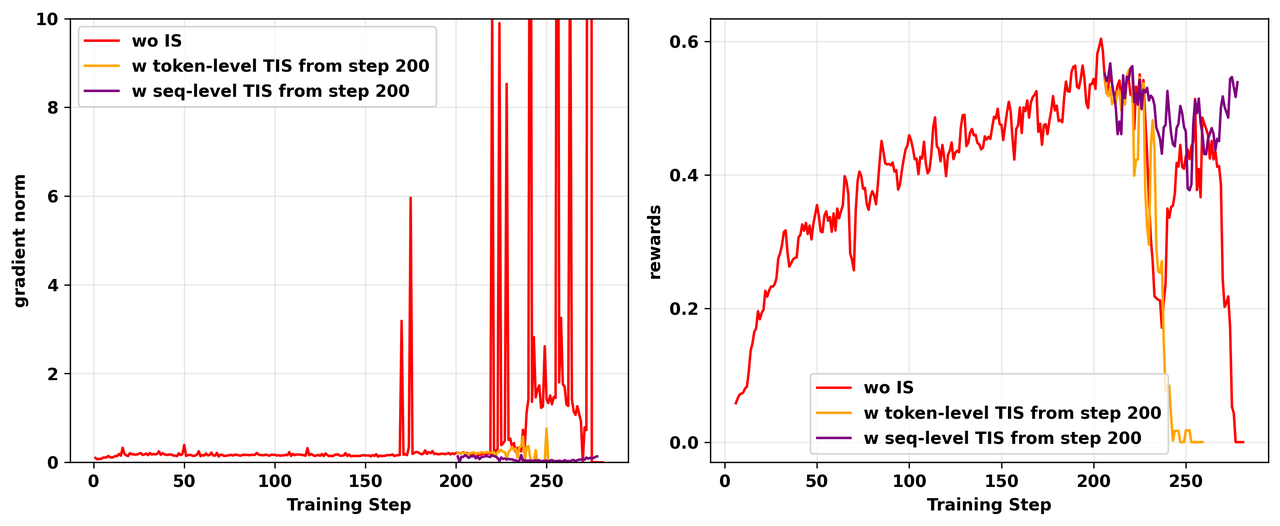
\includegraphics[width=\linewidth,height=0.64\textheight,keepaspectratio]{figures/image-20.png}
\caption*{\textbf{图 14。}不同 TIS 策略的消融实验。未使用重要性采样的原始同策略实验在 200 步后崩溃并出现梯度爆炸；另外两次实验分别从第 200 步恢复，并加入词元级 TIS 或序列级 TIS。左：梯度范数；右：训练奖励。}
\end{figure}


% source-block: 27b211a5-58b7-8016-9cb8-ff6f0de98a30 (sub_sub_header; source-index: 239)

\hypertarget{src-27b211a5-58b7-8016-9cb8-ff6f0de98a30}{}
\subsubsection*{推理强化学习中的词元级 TIS}


% source-block: 27b211a5-58b7-8039-9112-d72fa45bb16d (text; source-index: 240)

虽然词元级 TIS 在复杂 TIR 实验中失败，但对于不匹配较小的简单推理强化学习，它可以帮助防止崩溃。在同策略 GRPO 和 RLOO 实验中（图 15），词元级 TIS 避免了梯度爆炸；不过训练依然不稳定，也没有取得更好的最终性能，其潜在原因可能仍是梯度偏差。


% source-block: 271211a5-58b7-80a6-89b2-f5313ed260bf (image; source-index: 241)

\begin{figure}[H]
\centering
% source-block: 271211a5-58b7-80a6-89b2-f5313ed260bf (image)
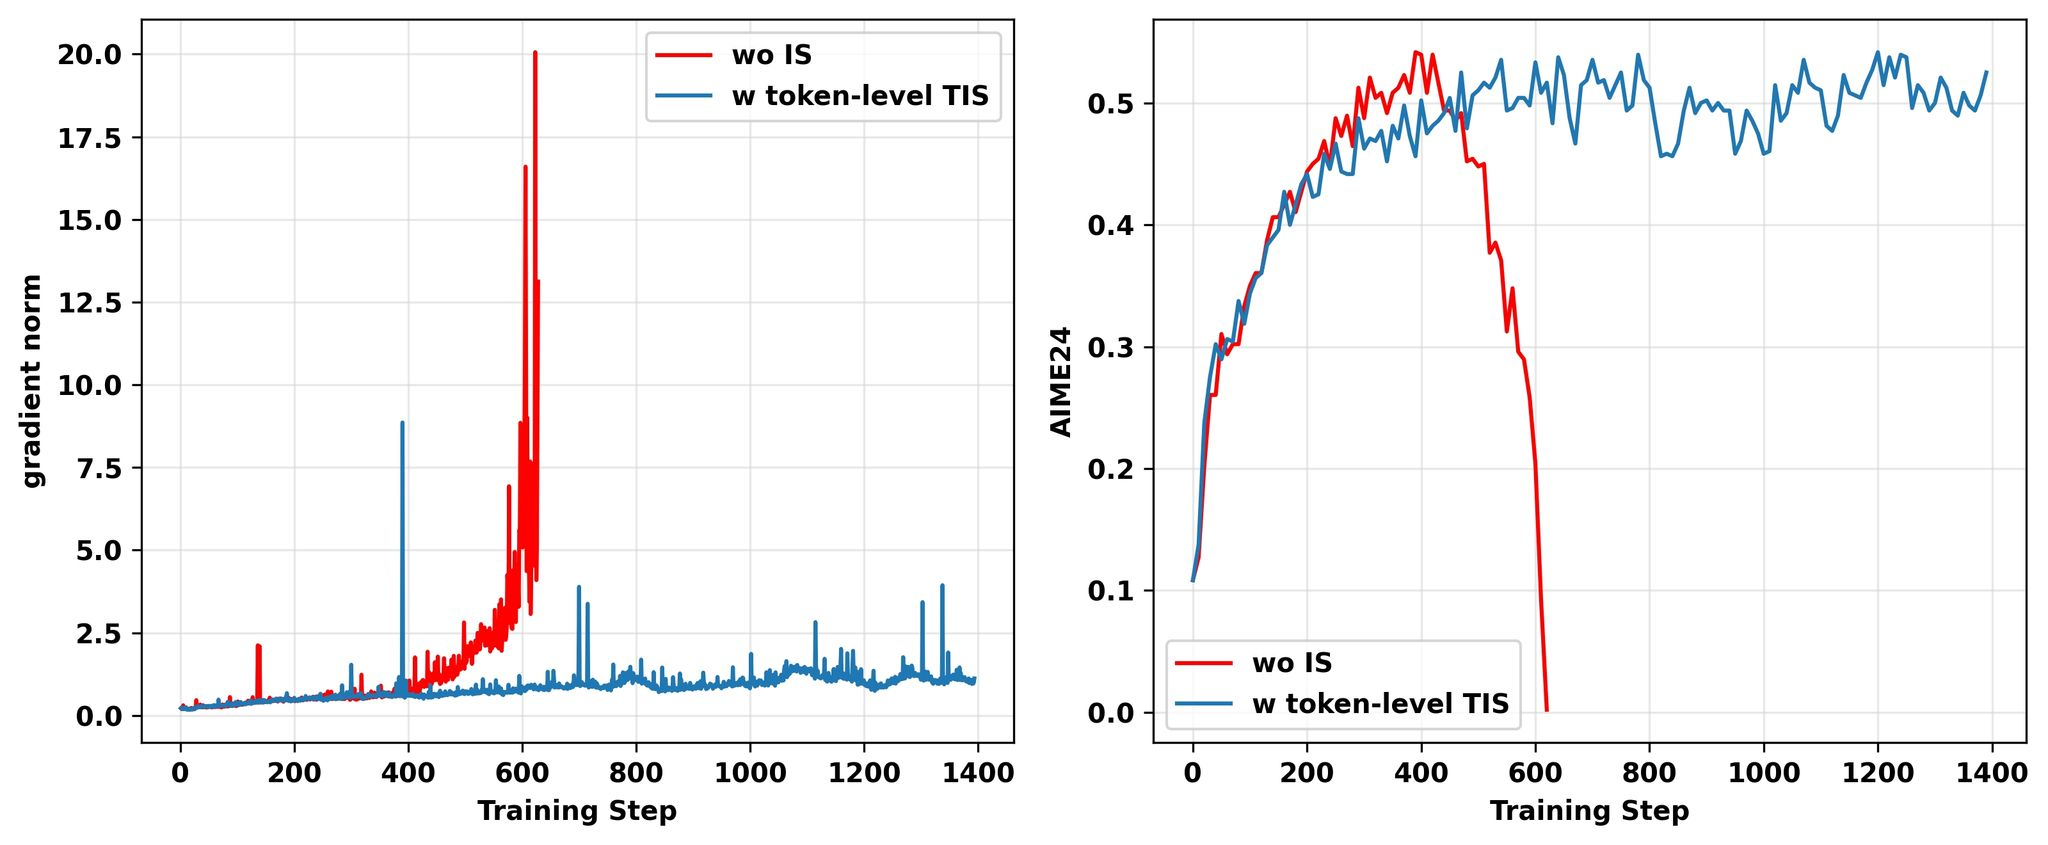
\includegraphics[width=\linewidth,height=0.64\textheight,keepaspectratio]{figures/image-21.jpg}
\caption*{\textbf{图 15(a)。}H100 上推理强化学习的同策略 GRPO 实验：不使用重要性采样，与使用词元级重要性采样（$C=2$）的比较。左：梯度范数；右：AIME24 准确率。词元级 TIS 避免了训练崩溃，但没有取得更好的测试性能。}
\end{figure}


% source-block: 27b211a5-58b7-80b6-8007-d80f67c22b85 (image; source-index: 242)

\begin{figure}[H]
\centering
% source-block: 27b211a5-58b7-80b6-8007-d80f67c22b85 (image)
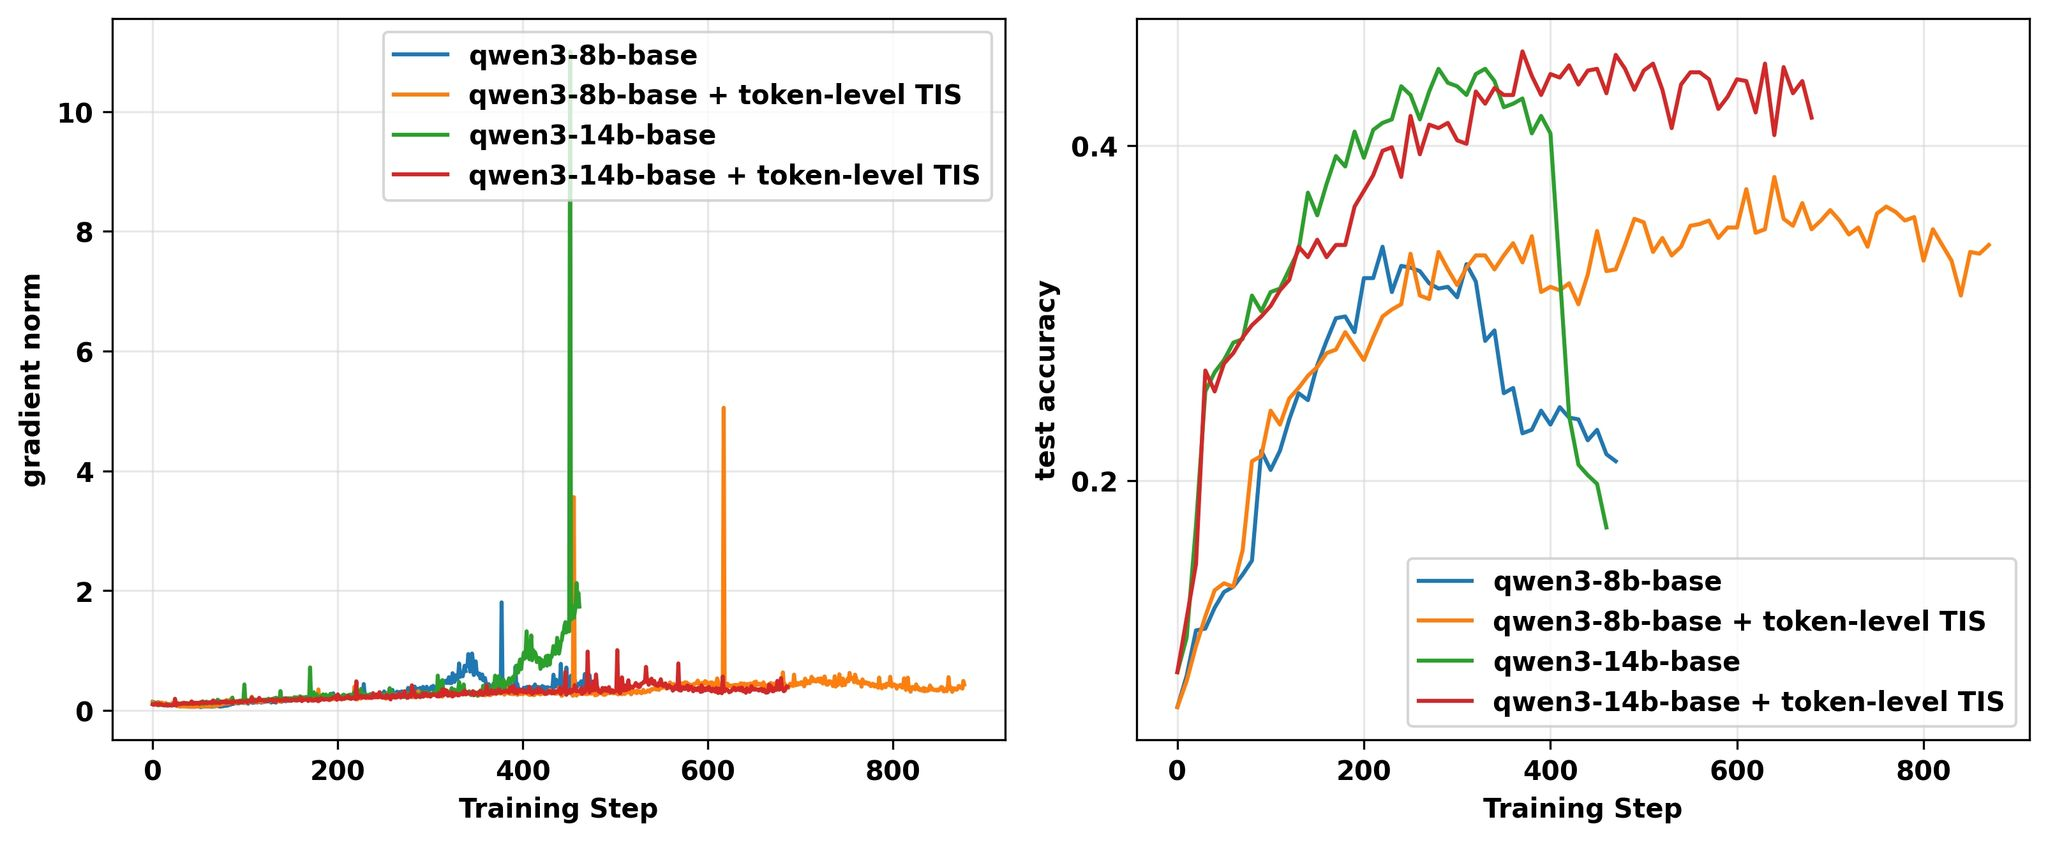
\includegraphics[width=\linewidth,height=0.64\textheight,keepaspectratio]{figures/image-22.jpg}
\caption*{\textbf{图 15(b)。}H100 上推理强化学习的同策略 RLOO 实验：不使用重要性采样，与使用词元级重要性采样（$C=2$）的比较。左：梯度范数；右：AIME24/AIME25 平均准确率。词元级 TIS 缓解了崩溃，但没有取得更好的测试性能，后期还有性能下降趋势。}
\end{figure}


% source-block: 27b211a5-58b7-809c-95f3-c38299424cb3 (sub_sub_header; source-index: 243)

\hypertarget{src-27b211a5-58b7-809c-95f3-c38299424cb3}{}
\subsubsection*{TIS 延长了训练，但仍可能不稳定}


% source-block: 27b211a5-58b7-8074-8280-d60a1f521829 (text; source-index: 244)

我们在 L20 GPU 上，从头开展使用序列级 TIS（$C=2$）的同策略 TIR 实验。如图 16 所示，虽然该方法避免了彻底崩溃，但奖励达到平台期后持续波动，测试性能也没有超过原始实验崩溃前达到的峰值。


% source-block: 27b211a5-58b7-80aa-abaf-e901a524bca8 (image; source-index: 245)

\begin{figure}[H]
\centering
% source-block: 27b211a5-58b7-80aa-abaf-e901a524bca8 (image)
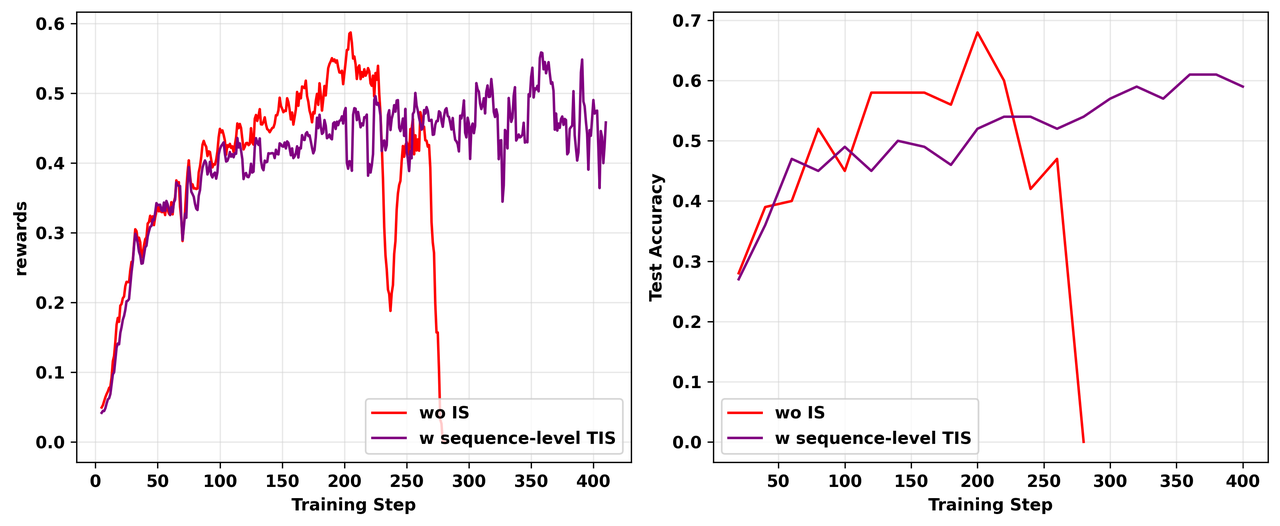
\includegraphics[width=\linewidth,height=0.64\textheight,keepaspectratio]{figures/image-23.png}
\caption*{\textbf{图 16。}不同 TIS 策略的进一步消融。未使用重要性采样的原始同策略实验在 200 步后崩溃；另一实验从头运行，配置相同，但加入 $C=2$ 的序列级 TIS。左：训练奖励；右：测试准确率。}
\end{figure}


% source-block: 27b211a5-58b7-8018-a714-c70402ddf952 (sub_sub_header; source-index: 246)

\hypertarget{src-27b211a5-58b7-8018-a714-c70402ddf952}{}
\subsubsection*{掩码重要性采样（MIS）}


% source-block: 27b211a5-58b7-80d0-a036-ddcfbe517351 (text; source-index: 247)

为改进 TIS，我们提出\textbf{掩码重要性采样（masked importance sampling，MIS）}：对重要性采样比率超过阈值 $C$ 的序列，将其策略损失掩掉，即 $\rho(y\mid x)\gets\rho(y\mid x)\mathbb I\{\rho(y\mid x)\le C\}$。图 17 表明，MIS 提高了训练稳定性，并在训练奖励和测试准确率上都超过了原始实验与 TIS 实验的峰值。\footnote{译注：原文正文强调稳定性的改善，而图 17 图注同时指出，MIS 和 TIS 在后期都仍存在不稳定性。译文保留两处表述，不能据此理解为 MIS 保证所有阶段稳定。}


% source-block: 27b211a5-58b7-808b-92f0-f53e0439f9d6 (image; source-index: 248)

\begin{figure}[H]
\centering
% source-block: 27b211a5-58b7-808b-92f0-f53e0439f9d6 (image)
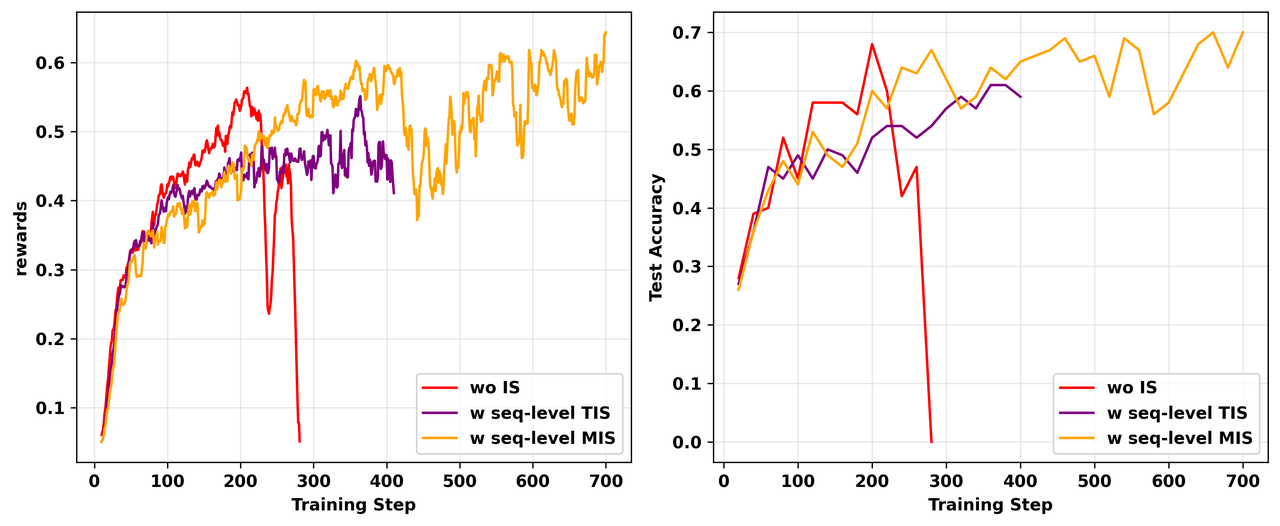
\includegraphics[width=\linewidth,height=0.64\textheight,keepaspectratio]{figures/image-24.png}
\caption*{\textbf{图 17。}L20 上同策略 GRPO 的序列级 MIS、序列级 TIS 与未使用重要性采样的原始版本对比。MIS 与 TIS 均延长了训练时间，但后期仍存在不稳定性。MIS 在训练奖励和测试准确率上均优于 TIS，并超过原始实验的峰值。左：训练奖励；右：测试准确率。}
\end{figure}


% source-block: 27b211a5-58b7-8051-a317-d40175e29b7a (sub_sub_header; source-index: 249)

\hypertarget{src-27b211a5-58b7-8051-a317-d40175e29b7a}{}
\subsubsection*{词元级 MIS 与序列级 MIS}


% source-block: 27b211a5-58b7-80c5-aac5-c904c8662cee (text; source-index: 250)

最后，我们比较了词元级和序列级 MIS。如预期，图 18 表明，虽然两者都避免了初期梯度爆炸，但词元级 MIS 实验仍然崩溃。这再次支持我们的结论：对于复杂、长时域的自回归任务，有理论依据的序列级修正更加可靠。


% source-block: 27b211a5-58b7-80a9-9837-dc6b5f980e1b (image; source-index: 251)

\begin{figure}[H]
\centering
% source-block: 27b211a5-58b7-80a9-9837-dc6b5f980e1b (image)
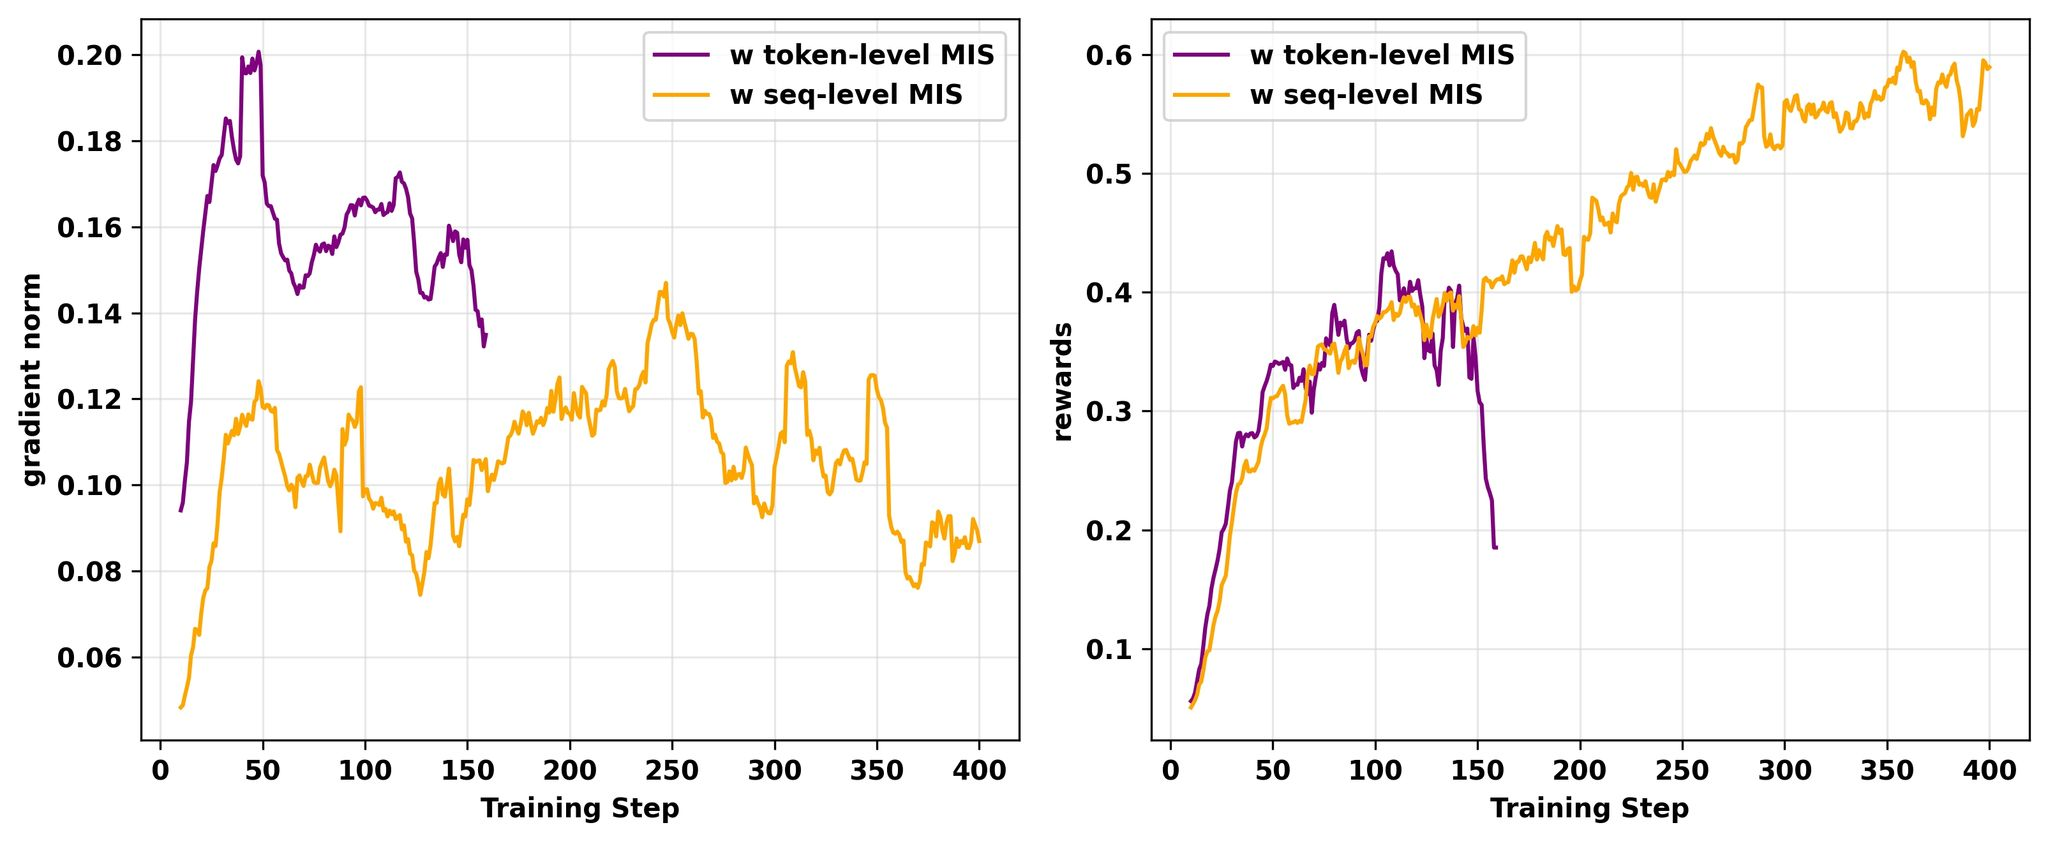
\includegraphics[width=\linewidth,height=0.64\textheight,keepaspectratio]{figures/image-25.jpg}
\caption*{\textbf{图 18。}L20 上同配置的同策略 GRPO：词元级 MIS 与序列级 MIS 的比较。左：梯度范数；右：训练奖励。}
\end{figure}


% source-block: 271211a5-58b7-80f8-a38a-dae34f381bef (sub_sub_header; source-index: 252)

\hypertarget{src-271211a5-58b7-80f8-a38a-dae34f381bef}{}
\subsubsection*{4.2.2 Top-$p$ 采样}


% source-block: 271211a5-58b7-809c-9cf7-ce530f69f705 (text; source-index: 253)

如前所述，vLLM 策略的低概率词元更容易遭受严重的训练与推理不匹配，使 FSDP 策略为其赋予极低概率。为进一步验证这一点，我们开展了 top-$p$ 消融实验。在 L20 GPU 上运行同策略 GRPO，将 vLLM 采样策略的 \code{top-p} 分别设为 0.98、0.99 和 0.999；这里没有使用重要性采样进行梯度修正。

通过减小 \code{top-p}，我们希望降低推理阶段出现极低 vLLM 概率词元的频率，从而缓解训练与推理不匹配。图 19 与预期一致：更小的 \code{top-p} 减少了 \code{vllm-kl} 尖峰。不过，更小的 \code{top-p} 也会增大 vLLM 策略 $\piv$ 与 FSDP 策略 $\pif$ 的分布差异。因此，在没有使用 TIS 时，梯度偏差增大，\code{top-p} 越小，奖励提升越慢。


% source-block: 271211a5-58b7-80a0-9f28-d37a3e81825e (image; source-index: 254)

\begin{figure}[H]
\centering
% source-block: 271211a5-58b7-80a0-9f28-d37a3e81825e (image)
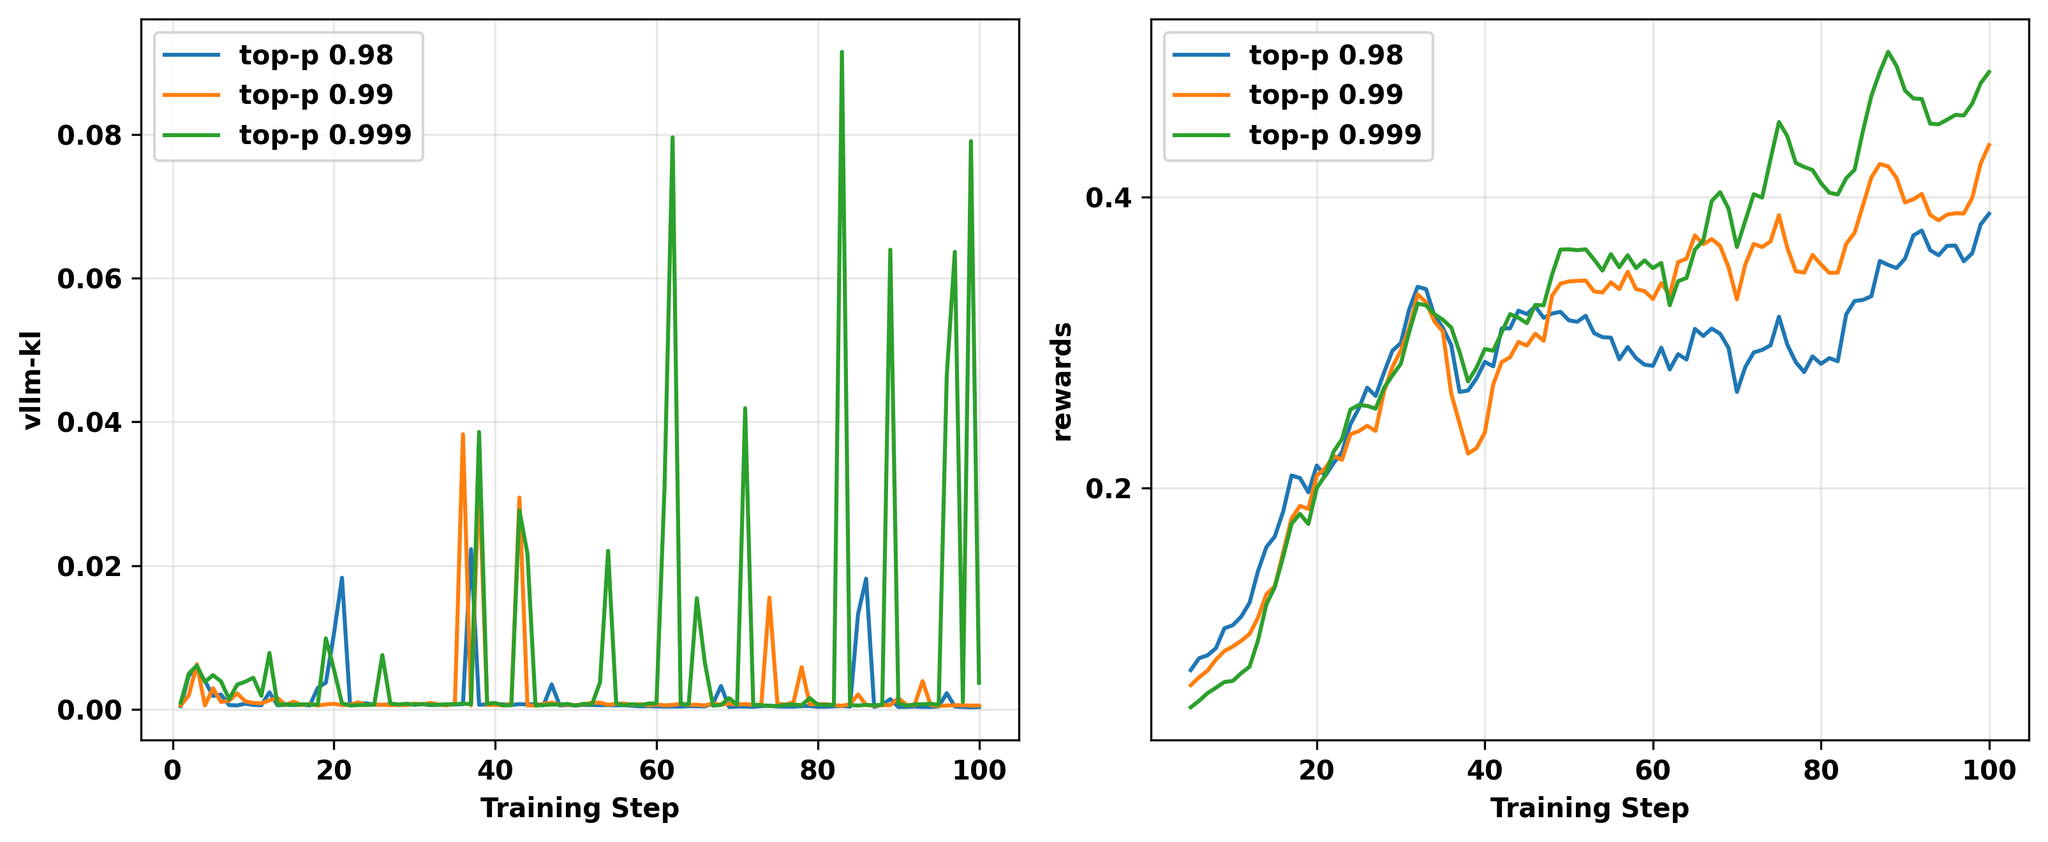
\includegraphics[width=\linewidth,height=0.64\textheight,keepaspectratio]{figures/image-26.png}
\caption*{\textbf{图 19。}强化学习中 vLLM 采样策略的 \code{top-p} 消融。同策略 GRPO 的 \code{top-p} 分别为 0.98、0.99 和 0.999。更小的 \code{top-p} 通常对应更小的 \code{vllm-kl}，但奖励提升也更慢。左：\code{vllm-kl}；右：训练奖励。}
\end{figure}


% source-block: 271211a5-58b7-8013-9729-e1f74e6c65ae (sub_sub_header; source-index: 255)

\hypertarget{src-271211a5-58b7-8013-9729-e1f74e6c65ae}{}
\subsubsection*{4.2.3 使用其他 GPU 系列}


% source-block: 271211a5-58b7-8099-83b6-cfe6b0b5c1e7 (text; source-index: 256)

发现 H20 上的训练与推理不匹配显著小于 L20 后，我们将所有 TIR 实验迁移到 H20，大幅减少了训练崩溃。图 20 展示了在完全相同配置下，分别使用 L20 与 H20 从头训练的两个同策略 GRPO 实验。H20 上的实验显著延长了稳定训练时间，并取得了更好的性能。


% source-block: 271211a5-58b7-8095-9c63-f3bcc7bbef56 (image; source-index: 257)

\begin{figure}[H]
\centering
% source-block: 271211a5-58b7-8095-9c63-f3bcc7bbef56 (image)
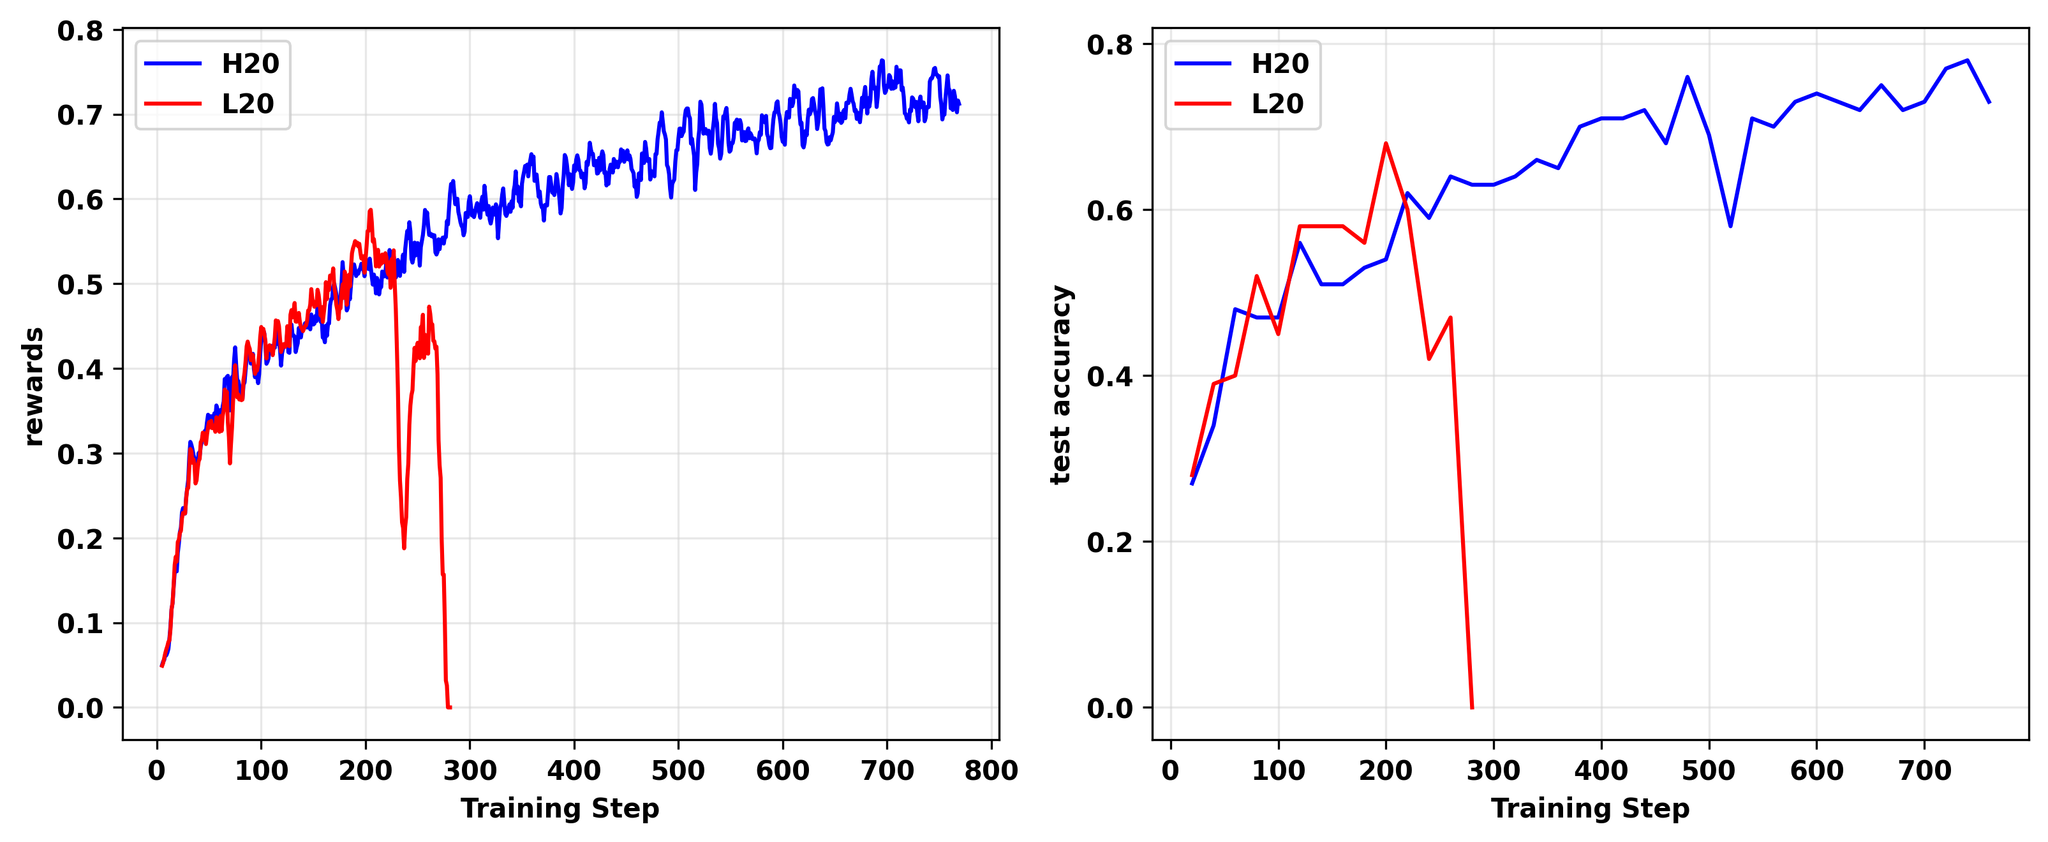
\includegraphics[width=\linewidth,height=0.64\textheight,keepaspectratio]{figures/image-27.png}
\caption*{\textbf{图 20。}分别在 L20 与 H20 上运行的两个同策略 GRPO 实验。左：训练奖励；右：测试准确率。}
\end{figure}


% source-block: 27a211a5-58b7-80fa-b2d9-d85708b21084 (sub_sub_header; source-index: 258)

\hypertarget{src-27a211a5-58b7-80fa-b2d9-d85708b21084}{}
\subsubsection*{4.2.4 关闭 vLLM 的级联注意力}


% source-block: 27a211a5-58b7-8064-b138-d3309bc466a0 (text; source-index: 259)

根据这个 \href{https://github.com/vllm-project/flash-attention/pull/87}{GitHub 讨论}，我们在初始化 vLLM 时设置 \code{disable_cascade_attn=True}，发现它能显著减小 A100 实验中的训练与推理不匹配。我们在 A100 上，以 Qwen3-14B-Base 为基础模型进行两个同策略 GRPO 实验，分别将 \code{disable_cascade_attn} 设为 \code{True} 和 \code{False}。图 21 表明，关闭级联注意力后，\code{vllm-kl} 从 $5\times10^{-2}$ 至 $10^{-1}$ 降至约 $10^{-3}$，不匹配大幅减小；训练集上的奖励也相应提高。


% source-block: 27a211a5-58b7-8082-b200-d1681ccb6ceb (image; source-index: 260)

\begin{figure}[H]
\centering
% source-block: 27a211a5-58b7-8082-b200-d1681ccb6ceb (image)
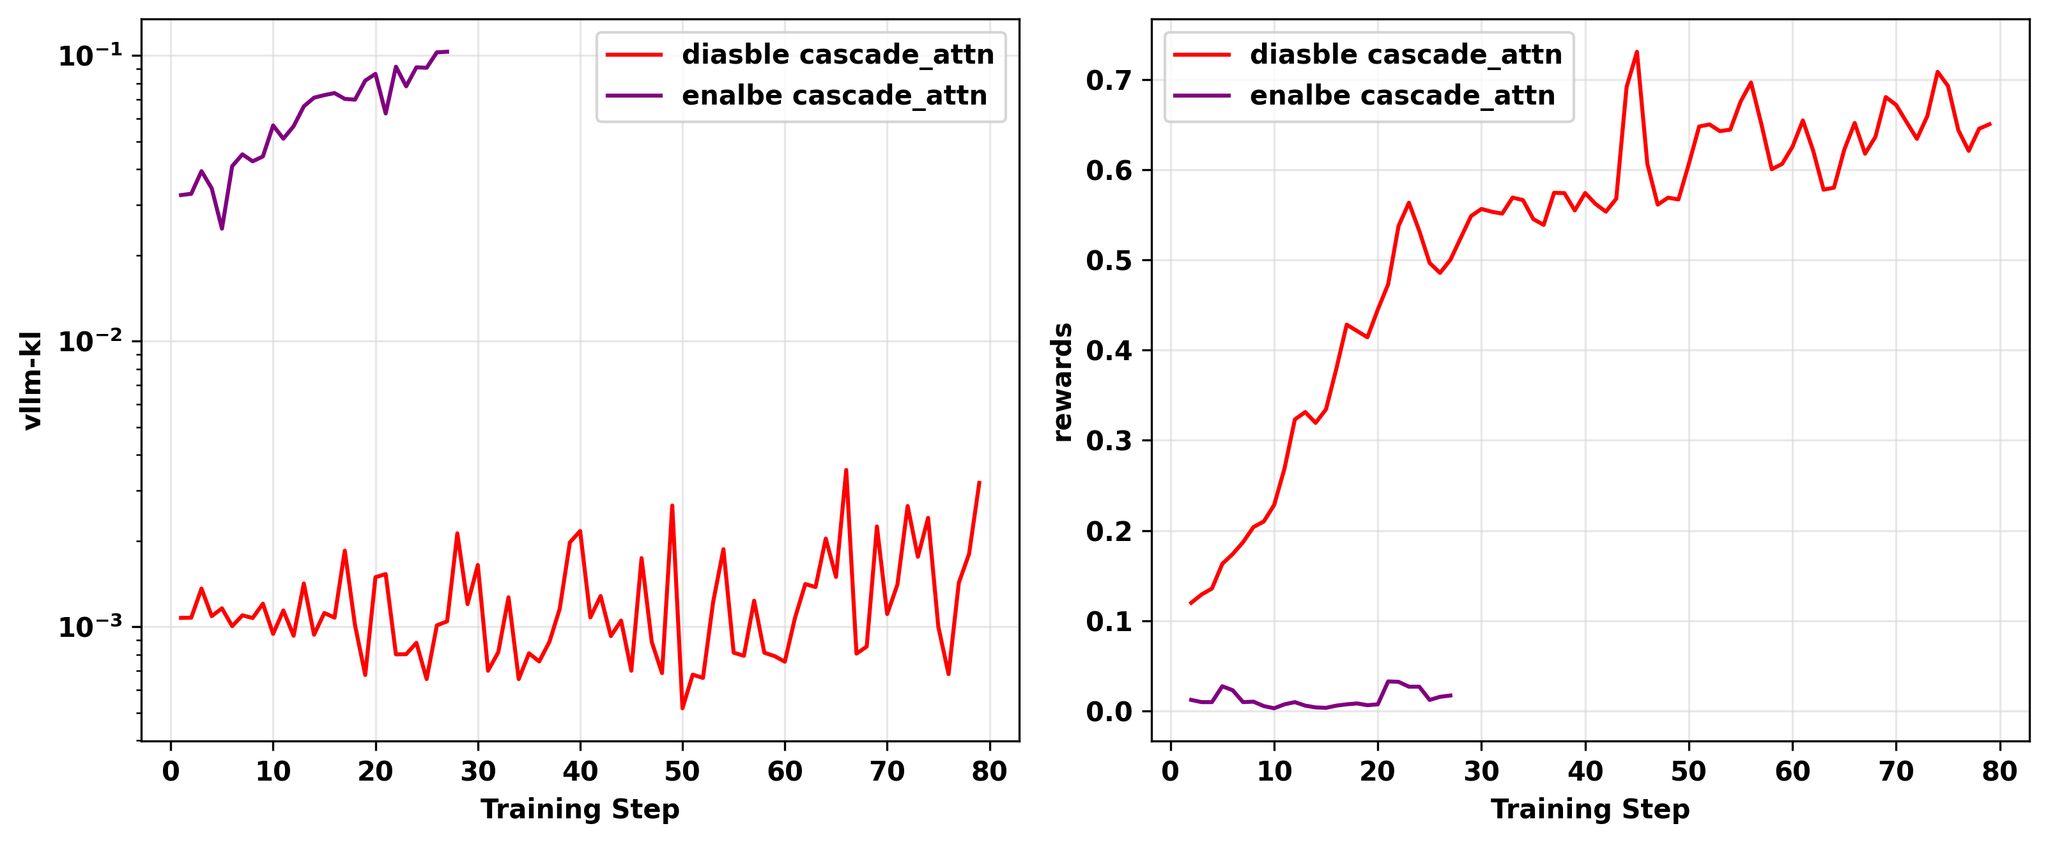
\includegraphics[width=\linewidth,height=0.64\textheight,keepaspectratio]{figures/image-28.png}
\caption*{\textbf{图 21。}级联注意力的消融实验。在 A100 上运行两个同策略实验：一个启用级联注意力，另一个使用相同配置但关闭级联注意力。左：\code{vllm-kl}；右：训练奖励。}
\end{figure}


% source-block: 277211a5-58b7-806a-8461-c2c69bf1c100 (divider; source-index: 261)
